\chapter{Introduction}

Over the last few decades, the rate of obesity and overweight people in the World has greatly increased. As presented for the UK case in the Fig. \ref{fig:obesity_uk}, the obesity rate has increased by 12\% between 1980 and 2013, and the overweight rate by 13\%. It is forecast by the World Health Organisation to continue to grow in the next decades.

\begin{figure}[h]
    \centering
    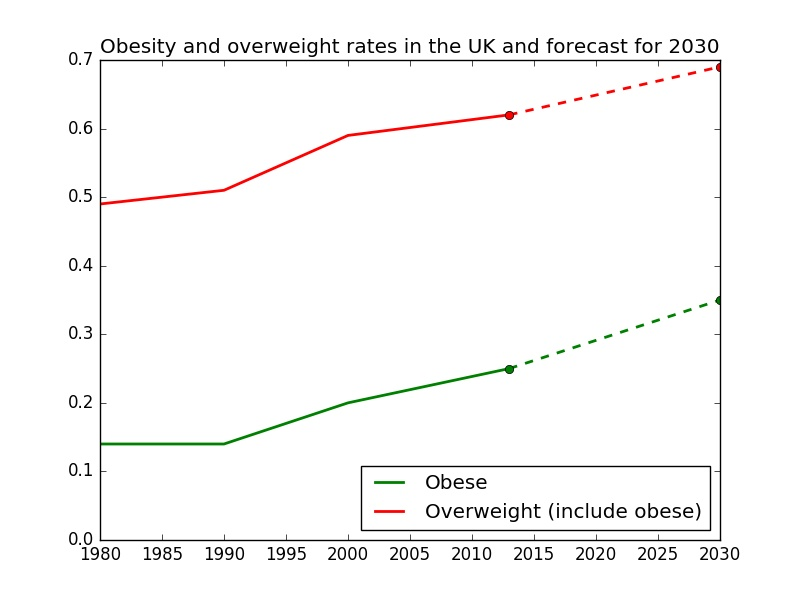
\includegraphics[width=0.5\textwidth,  height=0.455\textwidth ]{img/obesity_uk.jpg}
    \caption[Obesity and overweight rate of the adult population in the uk between 1980 and 2030. \textit{Source: World Health Organisation}]{Obesity and overweight rate of the adult population in the uk between 1980 and 2030}
    \label{fig:obesity_uk}
\end{figure}

Being \enquote{overweight} is defined as having a Body Mass Index (BMI) – a person's weight in kilograms divided by the square of his height in meters ($ kg / m^2 $) – of between 25 and 29.9, and \enquote{obese} by a BMI of 30 and above.

As stated in \cite{Mokdad2003}, obesity is strongly associated with several major health risk factors such as stroke, high blood pressure, type 2 diabetes and high cholesterol. Thus, it has a great human and economic (Zhang et al. \cite{Zhang2010} in 2010 showed 12\% of the total worldwide health expenditure is spent on diabetes and the total cost will continue to grow) cost for societies.

Associated with lifestyle changes, recording what we eat is one way to control our eating. Studies such as \cite{Burke2011a} show the benefit of reporting its daily diet to lose weight and improve the quality of its food intake. And more generally, it can be a way to treat eat disorders

Yet, manually recording detailed information regarding all meals is a tedious and time consuming task and it is hard for people to adhere to this process for a long time. Moreover, it often needs a trained patient. As presented in \cite{Lichtman1992}, user logs are prone to errors (users tend to underestimate its intake).

At the same time, image processing methods has greatly improved the recognition rate of elements in a picture. ImageNet is a dataset containing more than 1,2 million images split into 1000 classes. Since 2010, the yearly challenges include localisation, classification and detection. Numerous researchers, students, educators or information technology companies are participated.

As described in Fig. \ref{fig:imagenet_results} and using data from the challenge result report \cite{Russakovsky2015}, the mean classification error for each class and localisation has been greatly reduced between 2010 and 2014.

\begin{figure}[h]
    \centering
    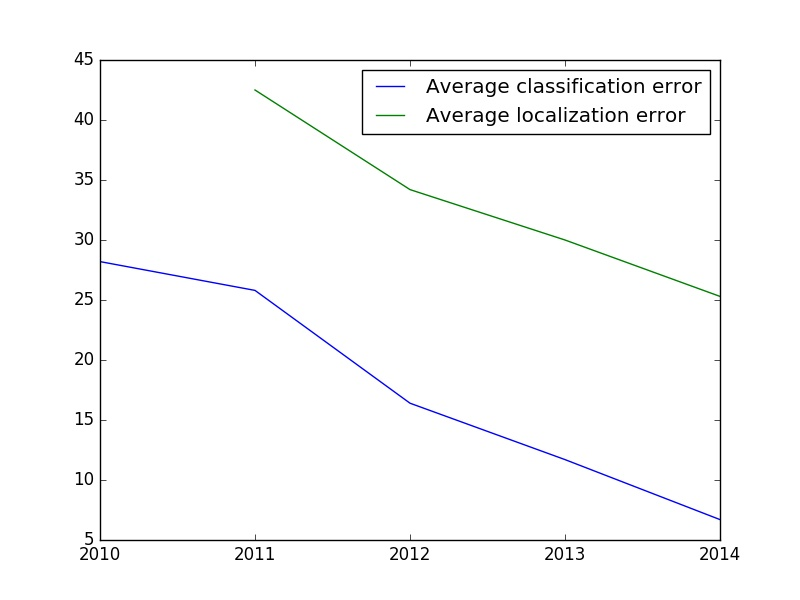
\includegraphics[width=0.5\textwidth,  height=0.455\textwidth ]{img/imagenet}
    \caption{Average classification and localisation error of the best results for different ImageNet challenges}
    \label{fig:imagenet_results}
\end{figure}

With the widespread use of smartphone, cameras or wearable devices, people can easily take pictures of a good quality and are already taking photos of their food and posting them on website such as Food Gawker, Instagram, Flickr or Yelp.

That's why, it has recently been proposed to automate the process and assist patient and their medical personnel (nutritionists, psychologists) to understand the patient's behaviour and habits. It extends the reach of care in a cost effective ways and counters some of the previous problem of manual report. It's part of the rise of e-healthcare / m-healthcare \cite{Hillestad2005, Menachemi2011}.

The idea is to have users who upload pictures of their daily meals to the application or website that constructs their food diary automatically. Using image processing, it estimates the dietary composition of the meal and keep record of the information for later viewing in formats such as tables or graphical representations.

Food recognition is a promising applications of image processing and machine learning. Its overall process is:
\begin{itemize}
    \item Extract key characteristics
    \item Localise food items if the application allow multiple food items
    \item Recognise the food
\end{itemize}

Feature description is essential to achieve good object detection and image categorisation. Preferably the method should be invariant of the conditions, i.e. the luminosity, orientation or scale of the picture.

In this thesis, we focus on the food recognition. It has already numerous challenges such as:
\begin{itemize}
    \item \textbf{high intra-class variability} : we can have high variability between pictures for the same particular kind of food items, due to:
    \begin{itemize}
        \item environmental conditions (e.g. luminosity, quality of the camera)
        \item plating (the way it is served)
        \item variation of the way the picture is taken: numerous transformation can be applied to a same picture (scale, translation, rotation, skewness, crop)
    \end{itemize}
    This is illustrated in Fig. \ref{fig:intra-class_variability} for pictures of kaya toast.
    
    \item \textbf{low inter-class variability} : we can have low variability between different type of food such as between clear and miso soup as showed in Fig. \ref{fig:inter-class_variability}.
\end{itemize}

This makes localisation, classification and retrieval of food images a difficult task for current state-of-the-art techniques, and hence a compelling challenge for image processing and machine learning researchers.

Thus, the thesis is dedicated to the investigation on some methods that were found in the literature. Many modi operandi exist and we focus on three different descriptors: colour and texture features, local feature using Bag-Of-Word representation and convolutional neural network. These methods are evaluated on UEC-FOOD 256 and compared to previous papers. The generation of this dataset was presented by \cite{Kawano2015} by Kawano et al. from the University of Tokyo in 2015.

\begin{figure}
    \centering
    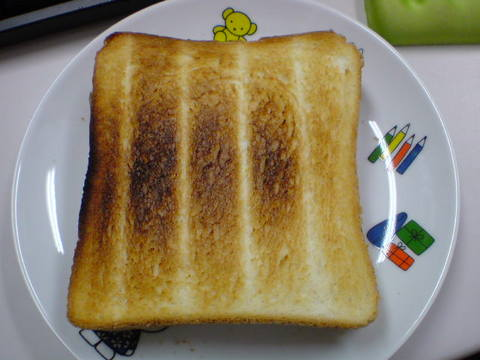
\includegraphics[height=4cm, width=4cm]{img/kaya_toast_1.jpg}
    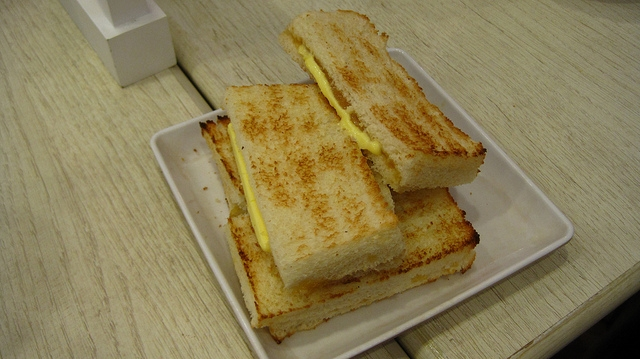
\includegraphics[height=4cm, width=4cm]{img/kaya_toast_2.jpg}
    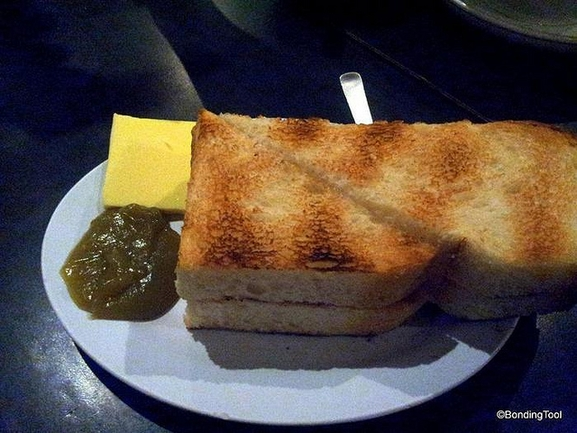
\includegraphics[height=4cm, width=4cm]{img/kaya_toast_3.jpg}
    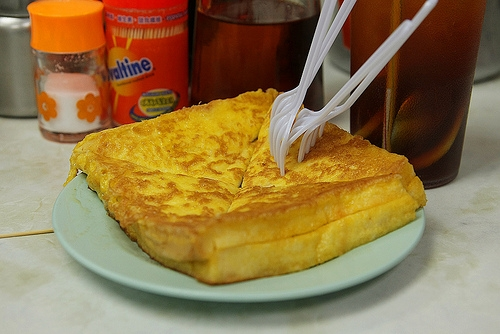
\includegraphics[height=4cm, width=4cm]{img/kaya_toast_4.jpg}
    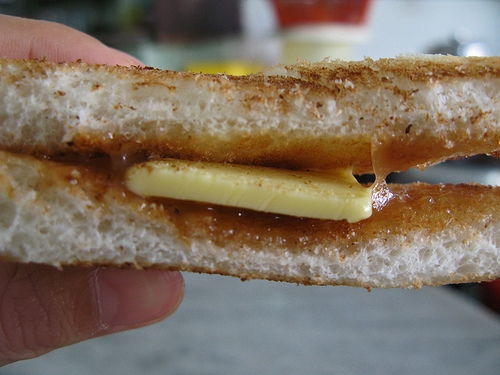
\includegraphics[height=4cm, width=4cm]{img/kaya_toast_5.jpg}
    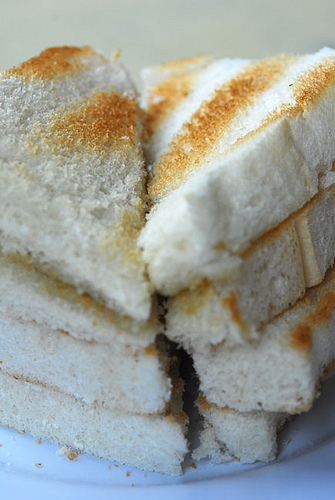
\includegraphics[height=4cm, width=4cm]{img/kaya_toast_6.jpg}
    \caption[Examples of high intra-class variability for kaya toast]{Examples of high intra-class variability for kaya toast. Pictures extracted from the UEC FOOD 256 dataset \cite{Kawano2015}.}
    \label{fig:intra-class_variability}
\end{figure}

\begin{figure}
    \centering
    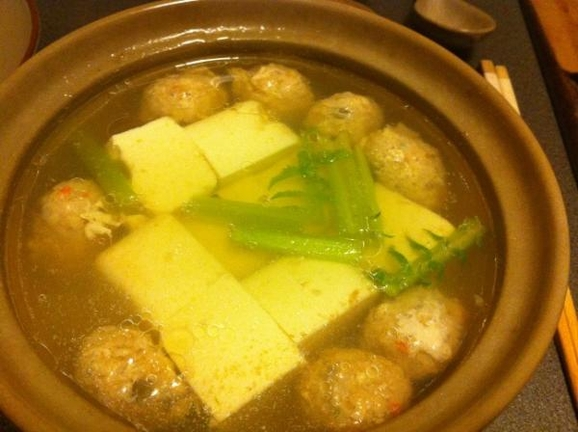
\includegraphics[width=7cm, height=6cm]{img/clear_soup.jpg}
    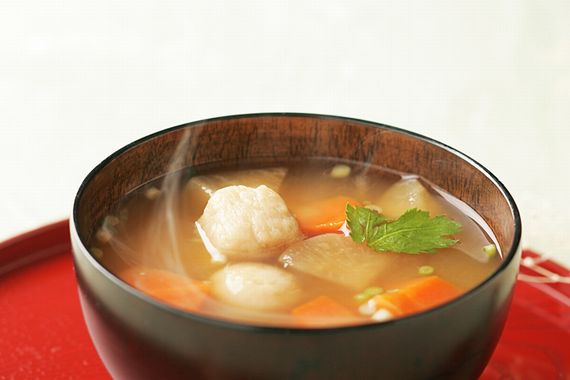
\includegraphics[width=7cm, height=6cm]{img/miso_soup.jpg}
    \caption[Examples of low inter-class variability for kaya toast]{Examples of low inter-class variability for clear soup (left) and miso soup (right). Pictures extracted from the UEC FOOD 256 dataset \cite{Kawano2015}.}
    \label{fig:inter-class_variability}
\end{figure}

The organization of this thesis is as follow. In section \ref{sec:previous_work}, previous work on food localisation, recognition and intake estimation is reviewed. Section \ref{sec:feature_descriptor} introduces the different image descriptors used, and in section \ref{sec:classifier} the classifiers are presented. In section \ref{sec:dataset}, the dataset is introduced. Section \ref{sec:evaluation} reports the experimental settings and results. Finally, in section \ref{sec:conclusion}, we draw the conclusion and state the limitation and possible future work.
